\documentclass[acmtog]{acmart}

\usepackage{makecell}
\usepackage{booktabs}
\usepackage{caption}
\usepackage{subcaption}
\renewcommand\cellalign{tl}
\def\BibTeX{{\rm B\kern-.05em{\sc i\kern-.025em 
b}\kern-.08emT\kern-.1667em\lower.7ex\hbox{E}\kern-.125emX}}

\begin{document}

\title{Towards Detecting Stalkerware Through Network Traces}


\author{Audrey Randall}
\author{Hugh Feng}
\author{Yu-Wun Wang}
\affiliation{\institution{UCSD}}

\begin{abstract}
Spyware is known as unwanted software that sends user state and information to 
an external party. Often these apps are not inherently malicious to the 
operating system and are thus difficult to detect. We explore a subset of 
spyware that are available in the Android Play store intended for spying on 
another person though his or her cell phone and create a new method of 
identifying their presence through network signatures.  
\end{abstract}

\maketitle

\section{Introduction}
In a world where technology now pervades every aspect of our lives, some 
aspects of our relationships with intimate partners have changed too. 
Specifically, when these relationships become abusive, there are more options 
available to the abuser for attempting to retain control over their partner. 
One of these options is the ability to install monitoring software on their 
partner's phone or computer to record their online activity, communications, 
and location. We refer to such software as ``stalkerware.''  

Stalkerware is not as widely studied as other types of malware, and much less 
information is available regarding it. Although it is superficially 
similar to other types of malware, there exist a few key differences. First, 
stalkerware is meant to be installed 
deliberately, by someone with physical access to the device that is to be 
monitored. In the context of intimate partner abuse, this presents an enormous 
threat. An abuser will often know or be able to coerce passwords to the device 
from the victim, making traditional defense measures irrelevant. This is one 
example of how traditional assumptions about security often do not apply in the 
context of IPV (intimate partner violence). Second, the 
threat model used by malware developers includes sophisticated antivirus and 
intrusion detection systems (IDSs). Both malware and stalkerware need to hide 
their presence on the target device, but malware is much more likely to 
attempt to obfuscate its network traffic. Stalkerware does not: it does not 
need to. Most antivirus does not detect apps capable of monitoring a target as 
potentially dangerous \cite{chatterjee_spyware_2018}. This presents an 
opportunity to glean information about stalkerware that is not available in the 
study of other forms of malware. Third, stalkerware falls 
for the most part into two categories: apps that are explicitly advertised for 
surveilling spouses and partners, and apps that have a different stated use but 
can be repurposed to stalk a target. These are usually marketed for theft 
prevention, finding lost devices, parental control of children, and employer 
control of employees. Previous literature refers to these as "dual-use" 
apps\cite{chatterjee_spyware_2018}. Some dual-use apps are ones that the 
victim wants to keep installed, such as 
``find my phone'' apps or social media apps that leak the user's location. The 
most troubling example of this is Facebook, which most victims want to keep 
so that they can contact their support network for help.  Determining if a 
particular dual-use app is being used for intimate partner surveillance (IPS) 
presents an enormous challenge. Given the wide spectrum of apps that can be 
used to facilitate IPS and the limited scope of this project, we chose to focus 
on more overt spyware.

Largely due to the differences between stalkerware and other malware, most 
available information on the \textit{pervasiveness} of stalkerware is anecdotal 
and piecemeal. Small-scale studies on how widespread spyware is do exist, but 
they have limitations. For example, in a survey of 72 
domestic violence shelters performed by NPR in 2014, 85\% said they worked with 
survivors whose abusers had tracked their location using their smartphone's 
GPS. 75\% said they have worked with clients who have had their conversations 
monitored by hidden stalkerware apps.\cite{shahani_smartphones_nodate} However, 
this study does not report how many individual clients experienced being 
digitally stalked. Additionally, it and similar work relies on 
reports from domestic violence shelters and health workers, which do not give 
a complete picture of the situation. Little to no data exist regarding spyware 
use on IPV victims who never visit a shelter. Traditionally, antivirus vendors 
collect metrics about 
malicious software, but antivirus often does not detect spyware 
\cite{chatterjee_spyware_2018}. Alarmingly, the stalkerware 
websites themselves claim to have hundreds of thousands of downloads per app, 
but these numbers are not likely to be trustworthy. The goal of this work is 
therefore to identify a means of identifying stalkerware in the wild so that it 
can be enumerated. We identified unique signatures in the traffic of 24 
stalkerware apps, by examining a traffic features such as domain names, HTTP 
header fields, protocol, and server name indicators (SNIs). For a complete 
list, see section \ref{network_signatures}. These signatures can be used by 
antivirus software and IDSs to determine how widespread stalkerware is. We show 
that these signatures are distinguishable from ordinary smartphone 
network traffic. We also propose a simple method of generalizing our signatures 
to spyware that we did not manually examine, and evaluate its robustness.


We began by identifying a set of apps that appear to be 
marketed primarily for IPS. We focused exclusively on Android apps, since our 
two test phones were both Androids. Apps that appear in Google searches for 
terms like 
"catch a cheating spouse," use vague language that appear to be marketed 
towards IPS, and label themselves as "spyware" became candidates that we 
considered. Overt spyware is not generally available from the app store - it 
must be downloaded from the manufacturer sites. It also costs much more than a 
typical app, with monthly 
subscriptions ranging from \$12 to \$70 per month. The exception is an app that 
we call SpyToMobile, which survives on the app store by frequently 
``reskinning'' itself (see section \ref{reskinning}).  
We selected several of these to test. All of these apps brand themselves as 
spyware and advertise that their products are undetectable on the target phone, 
despite also having disclaimers in small text that their software should not be 
used for any illegal activity. Some use language that appears designed to 
appeal to abusers. For example, underneath one promotional 
video, the app TheOneSpy has the disclaimer: ``Note for this video: Don't 
confuse with the world `Loved Ones' as spouse or Girl friends! Word Loved ones 
has used for kids and teens.'' Many of these apps also refer to the tracked 
phone as the ``target'' phone, and advertise that once installed, the app is in 
``stealth mode,'' meaning completely undetectable. None of these required 
rooting the phone. When installed, they ask for all the permissions they 
require, including device administrator privileges. They are capable of 
blocking incoming calls, recording messages that have been deleted, recording 
the screen of the phone using accessibility features, monitoring apps such as 
Facebook, WhatsApp, Kik, and Viber, and more.

Other apps were overt spyware, but nevertheless available from the Play Store. 
They fell into two categories: spyware that reskinned itself to appear to be 
many different apps, and apps designed for parents to keep track of children 
(or in one case, for adult children to track elderly parents.) For the most 
part, this latter category was offered by antivirus companies such as Avast and 
Norton. These apps offered 
multiple features, such as call screening, blocking Google search results, 
recording text messages and call logs, and ``panic buttons'' that would allow 
the surveilled phone to contact the surveillant and raise an alarm. They do not 
hide their app icons and generally make an effort to notify the user that the 
monitoring app is installed on their phone. The spyware that did not notify 
users of its presence mostly consisted of one app, called SpyToMobile, that was 
provided on the Play Store under many different names (see section \ref{}). 

We also identified many apps that were designed to track location or text 
messages, but were less comprehensive than the overt, off-store spyware. They 
track one feature each instead of tracking location, communication, and 
browsing history all at once. For the most part, these apps were free and 
available on the Google Play Store. Most of these were designed to keep track 
of the locations of the users' friends. 

\section{The Stalkerware Ecosystem}
Some spyware has a notification that the app is running, but that can be 
disabled. Those ones don't hide their icon, but you might have to go to All 
Apps to find it.
\subsection{The Practice of ``Reskinning''}
\label{reskinning}

\begin{figure*}
	\centering
	\begin{subfigure}{0.8\columnwidth}
		\centering
		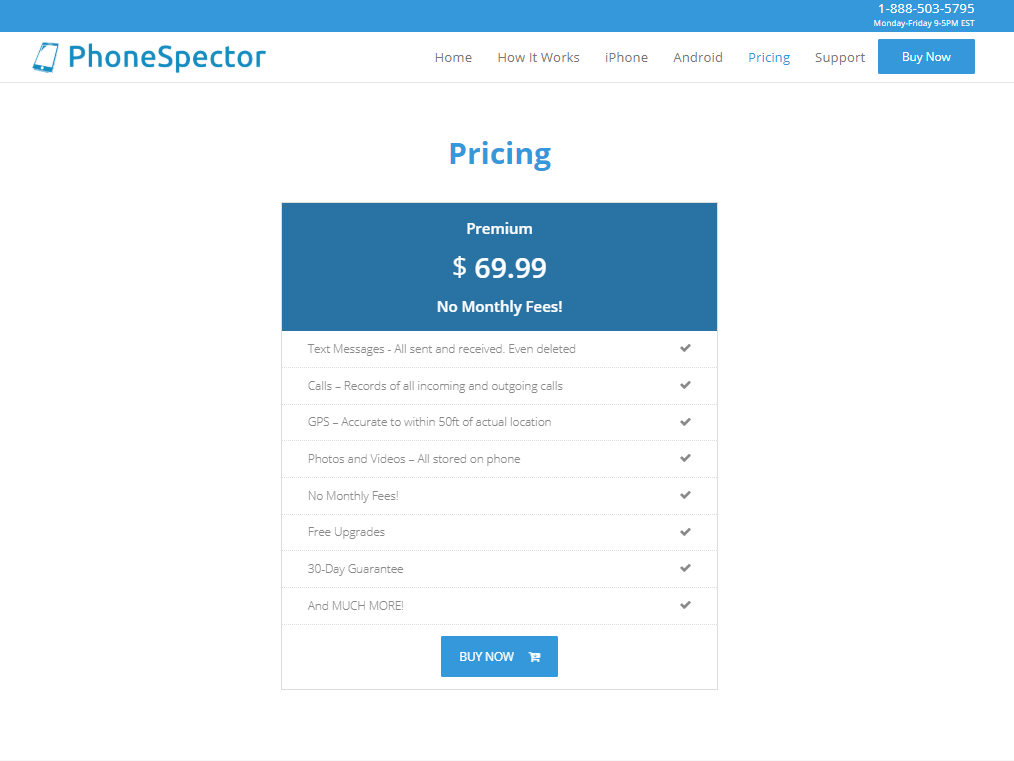
\includegraphics[width=0.9\linewidth]{../images/phonespector_small.png}
		\caption{PhoneSpector's pricing page }
		\label{fig:phonespector}
	\end{subfigure}%
	\begin{subfigure}{0.8\columnwidth}
		\centering
		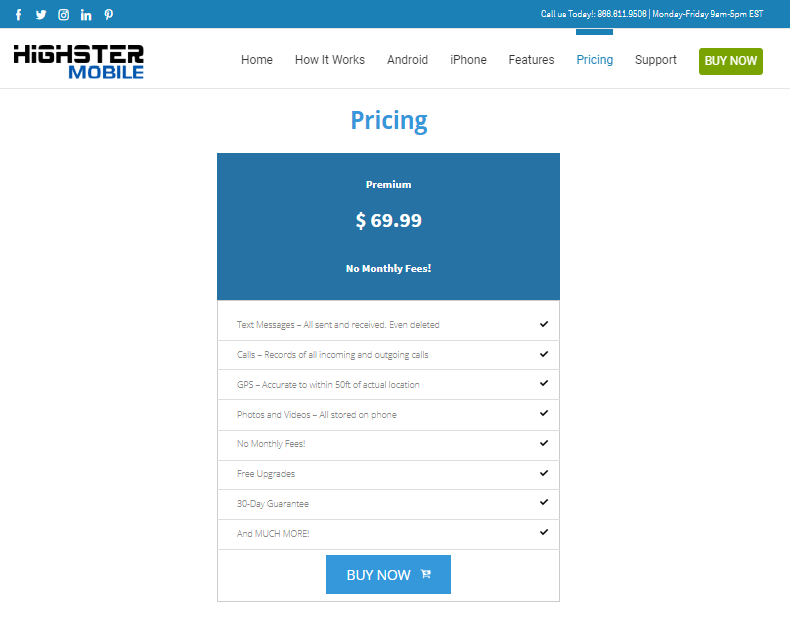
\includegraphics[width=0.9\linewidth]{../images/highstermobile_small.png}
		\caption{Highster Mobile's pricing page}
	\end{subfigure}
	\caption{PhoneSpector and Highster Mobile's payment pages. Although 
	PhoneSpector claims to be made by PhoneSpector LLC and HighsterMobile is 
	supposedly made by the Powerline Group, further investigation proved they 
	were the same company.}
	\label{fig:ilfmobiles}
\end{figure*}

As previously mentioned, spyware has a high turnover rate on the Google Play 
store, which leads to a practice we refer to as “reskinning:” a single app will 
be posted under many names, icons, and manufacturer names. Presumably, 
manufacturers do this because spyware gets reported frequently and taken down - 
we have already seen one instance of a spyware app getting removed from the 
Play store while we were examining it. Overt stalkerware which is not available 
through Google Play has also turned out to use reskinning, for reasons we 
haven’t yet discovered. Apps can frequently be identified as copies of each 
other by observing their dashboards (where users view the communications and 
locations of the target phones), download sites, and advertisements. Several 
groups of off-store apps have nearly identical websites, in terms of 
organization, color, fonts, placement of buttons, prices, and other factors. 
For example, the “ILFMobile group” consists of three different companies 
(ILFMobile, PowerLine Group, and PhoneSpector) that claim to make a total of 
four different apps. Further investigation showed that all three companies had 
the same physical address in addition to identical websites. Unfortunately, 
they also had identical bugs in their payment methods, so we were unable to 
purchase the apps and verify that their network traces were identical. Other 
app sites appear to be similar to each other in other ways, 
with many having a large panel with a darkened image background extolling the 
features of the app above two buttons, one for a "live demo" and the other to 
"buy now." This is somewhat circumstantial evidence - it is entirely possible 
that these manufacturers simply chose similar web templates, or copied each 
other's site in an attempt to undercut competition. We therefore confirmed our 
suspicions by checking if the traffic signatures were also similar. These 
reskinned programs are potentially a boon to 
our investigation as the identical network signatures make it more likely that 
one signature generalizes across multiple apps. We have identified the 
following groups of applications that appear to be reskinned versions of each 
other.
\begin{enumerate}
	\item \textbf{SpyToMobile group}: Employee Work Spy by Piter Cline, SMS 
	Tracker by TheHar, Mobile Tracking by Antwat, Cell Phone Tracker by Susdel, 
	and Texting, Chat, 
	Phone Spy by MaxLo. All of these apps download the same program, which is 
	called SpyToMobile. Any app from this group installed after the first 
	states ``SpyToMobile is already installed.''
	\item \textbf{ILFMobile group}: HighsterMobile, PhoneSpector, Auto Forward 
	Spy, Surepoint Spy, and EasySpy. We were unable to purchase these and 
	ensure that they have the same signatures due to a bug in their payment 
	system that prevented us from purchasing them.
	\item \textbf{Codero group}: HelloSpy and TheTruthSpy have identical 
	network signatures as well as nearly identical websites.
	Spyzie group: Spyzie and SpyMyFone also have identical network signatures 
	as well as identical websites.
	\item \textbf{CallSMSTracker group}: Call and Message Tracker by Remote 
	Karath and Cell Tracker by Trackme. These apps have identical dashboards 
	and contact the same domains.
\end{enumerate}
We cannot guarantee that we have identified all of the members of any 
particular group. If we have not, it will make other members easier to 
identify, since signatures we have already found will scale to identify more 
apps than we had time to download and manually examine.

\subsubsection{SpyToMobile}

\begin{figure}
	\centering
	\begin{subfigure}{0.5\columnwidth}
		\centering
		\includegraphics[width=0.9\linewidth]{../images/CellPhoneTracker.png}
		\caption{SpyToMobile's setup page }
		\label{fig:sub1}
	\end{subfigure}%
	\begin{subfigure}{0.5\columnwidth}
		\centering
		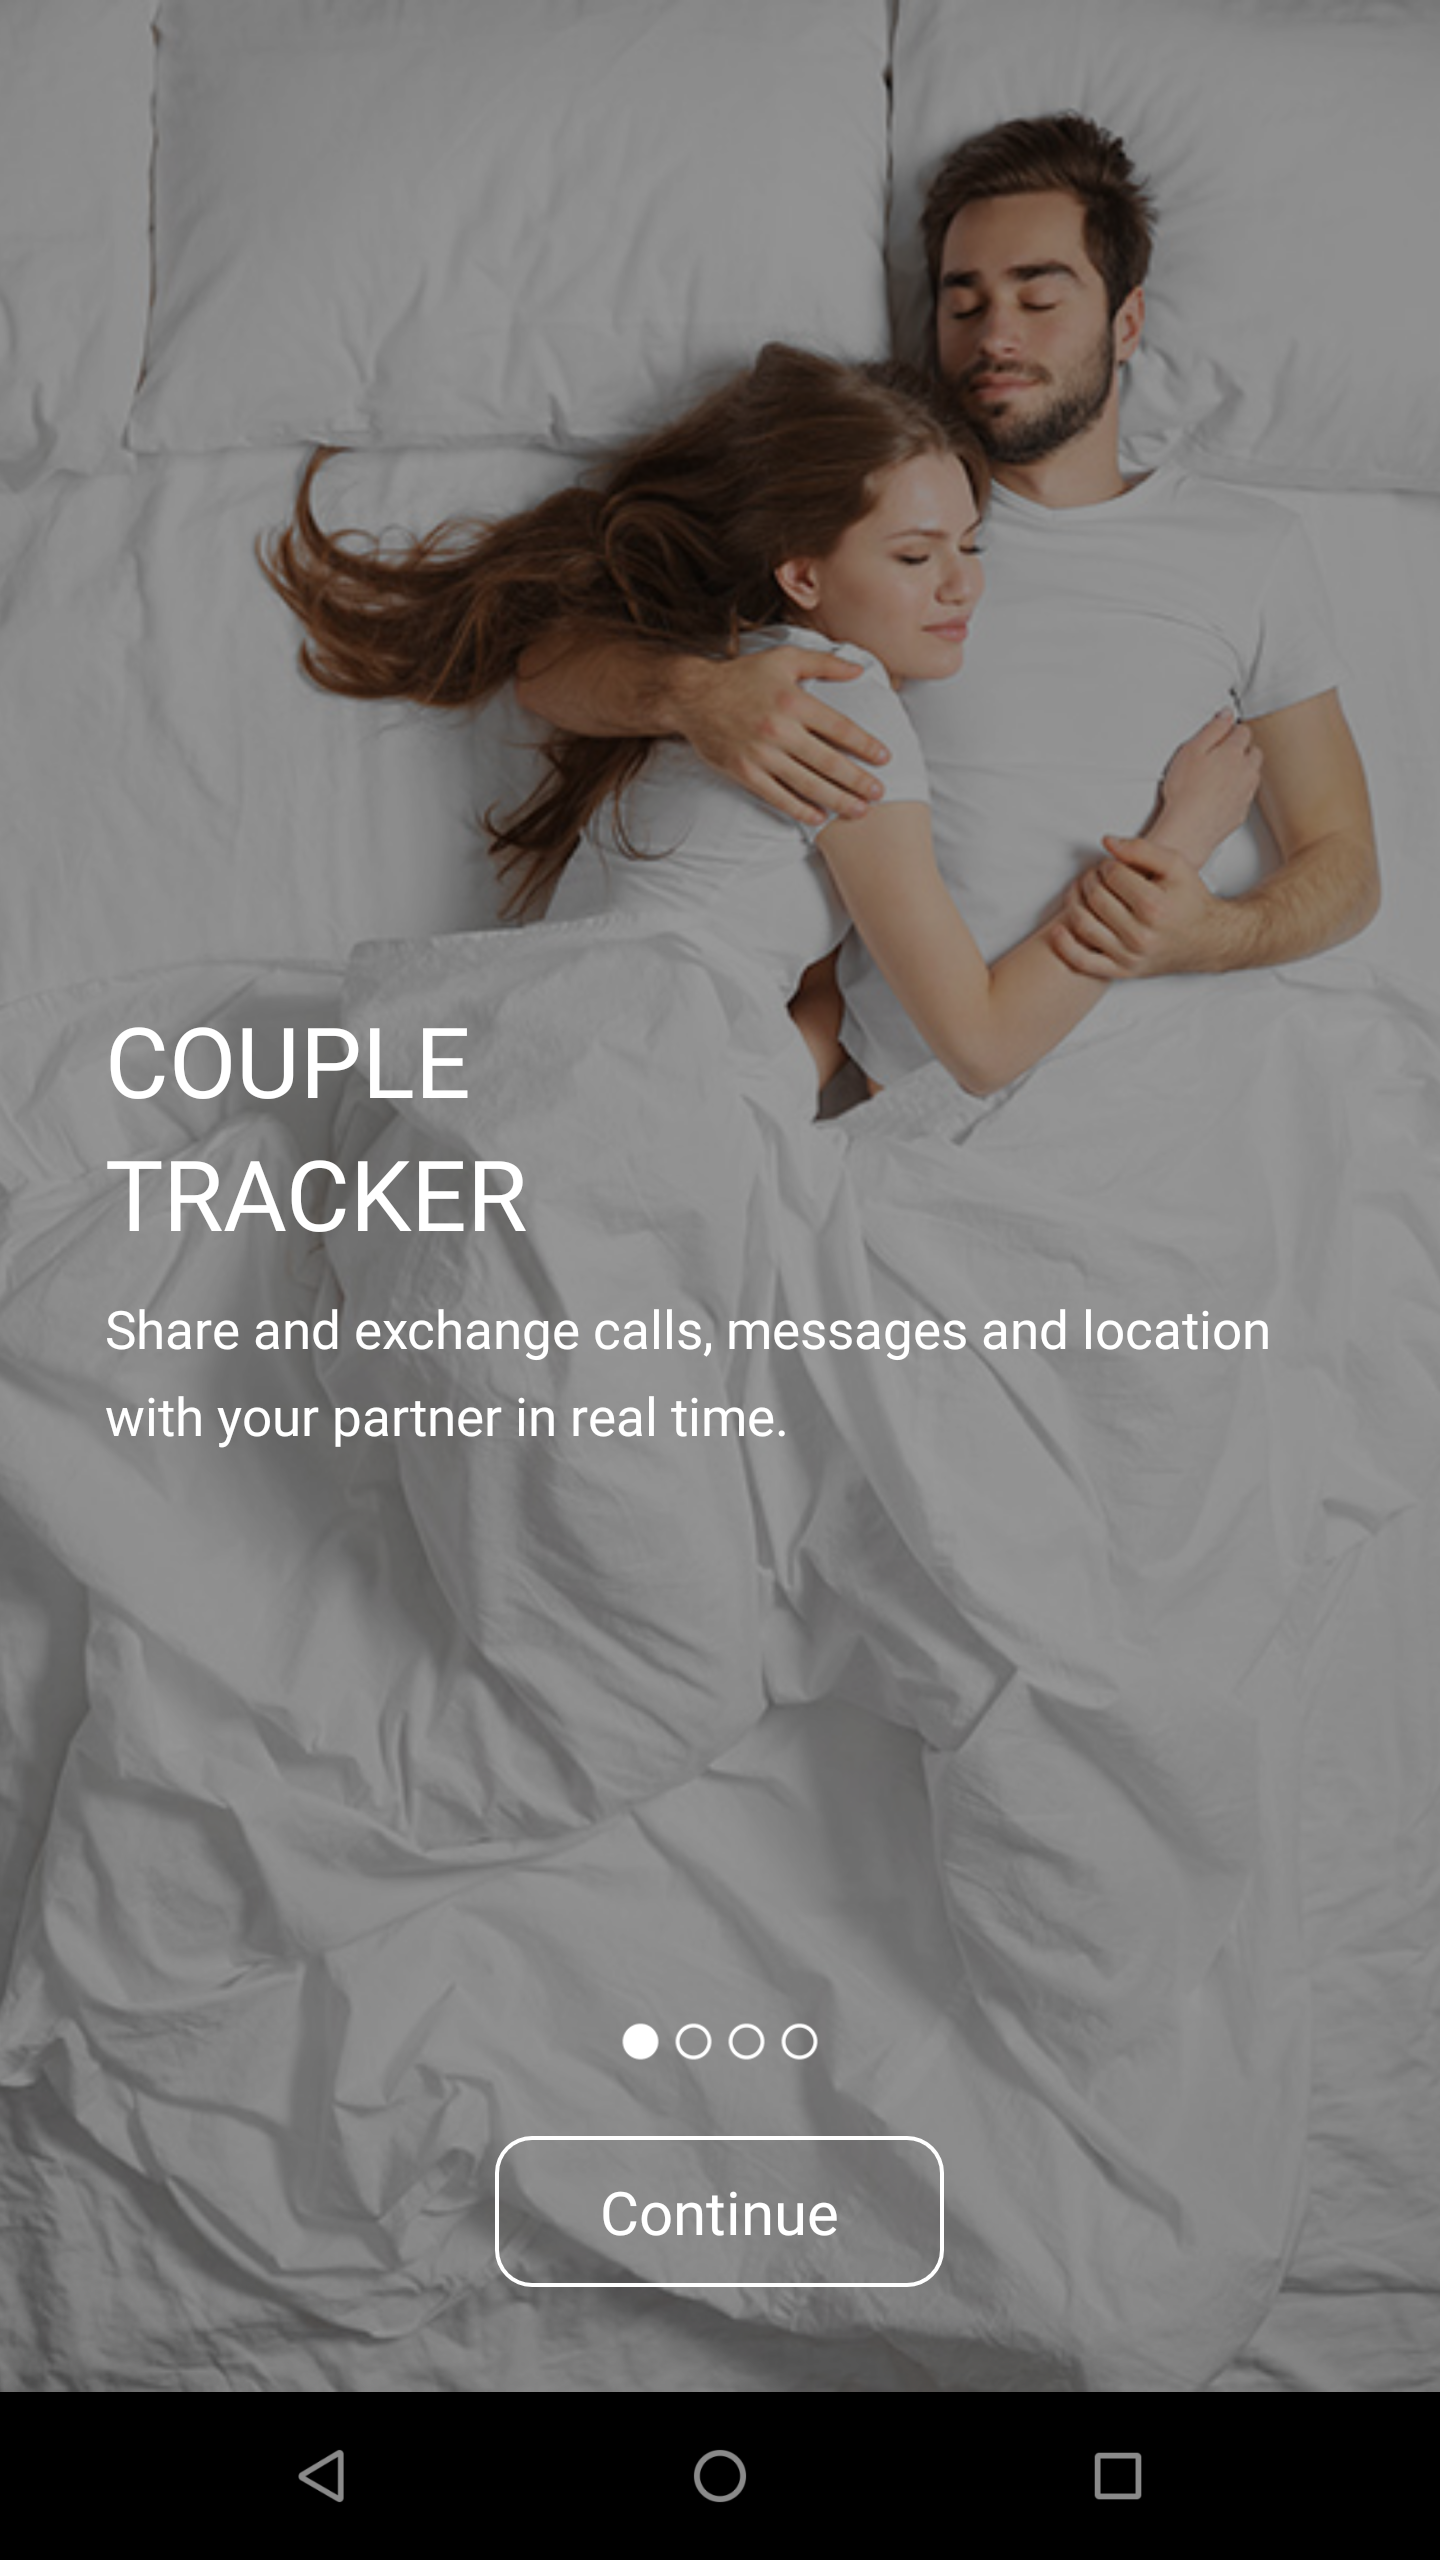
\includegraphics[width=0.9\linewidth]{../images/CoupleTrackerSetup.png}
		\caption{One of the setup pages for Couple}
		\label{fig:sub2}
	\end{subfigure}
	\caption{SpyToMobile and Couple's similarities. All SpyToMobile copies have 
	the same setup screen as \ref{fig:sub1} as well as identical signatures. 
	Couple did not share signatures with SpyToMobile.}
	\label{fig:spytomobile_couple}
\end{figure}


SpyToMobile is an interesting case 
because it fits the description of a generic stalkerware app so closely that it 
is the perfect example of spyware on the Play Store. Moreover, this single app 
has been repackaged multiple times. We have discovered that there have been at 
least six copies of the app on the Play store while our work has been ongoing, 
all with different developers and 
different names. We also found that the same image SpyToMobile uses in its 
"downloading" screen is used in another app, which had no similarities among 
its network signatures, called Couple. Figure \ref{fig:spytomobile_couple} 
shows the similarities.

\subsection{Competition Among Manufacturers}

App manufacturers appear to be well aware of their competition. When the term 
``hello spy'' is typed into Google Search, ads appear captioned ``Hellospy | 
See All Phone Data Remotely | mSpy.com'' and ``HelloSpy - Free Download | \#1 
Phone Tracker Software\&App | spymyfone.com.'' Clicking on these leads the user 
to the download pages for mSpy and SpyMyFone respectively, not the site for 
HelloSpy. Based on network traces and website appearances, we do not believe 
any of these three apps are made by the same manufacturer. Spyware groups also 
create “review” websites that review their own products, posing as third party 
spyware enthusiasts. At least one blog that is supposedly run by 
an independent party reviewed apps that coincidentally were all made by the 
ILFMobile group\cite{noauthor_best_nodate}. This blog reviews the 
“top 5 cell phone spy apps,” all of which are ILFMobile’s own apps, on a 
website called “bestcellphonespyapps.com.” We haven’t determined what advantage 
spyware manufacturers derive from appearing to make more apps and competing 
with themselves.

Somewhere: put a note about the weird thing where the paid apps try to make you 
download stuff again. Maybe it's just us? Maybe they're trying to boost 
download count?



\subsection{App Quality}

The other category for stalkerware encompasses a large range of quality. Many 
apps advertised as stalkerware have absolutely no functionality other than 
advertisement of other apps. The few that are functional are often simplistic 
in both features and network patterns. Unlike the overt apps, however, the vast 
majority are usually free with advertisements. 

\section{Related Work}
Previous studies [1,2], the media [3,4], and intimate partner violence (IPV) 
survivors have all reported that spyware is becoming an increasing source of 
intimate partner surveillance (IPS). Tracking functions supported by spyware 
allow stalkers to monitor communications, track locations, and remotely 
activate cameras and microphones [3,4]. In Dr. Ristenpart’s work [5], they 
proposed methods for searching IPS-related apps. By Google search query 
expansion and unsupervised classification, they collected 9,224 apps possibly 
related to IPS on Google play and open-web. They manually selected 70 apps for 
investigation. They observed the most fundamental functions of these apps are 
monitoring locations, communication logs and data, media contents, and phone 
usages. They also found that existing anti-spyware tools cannot effectively 
detect IPS-related apps.
Mobile apps are often identified via the User-Agent string of the HTTP request, 
when one is available [7]. With the increased use of HTTPS this may not always 
be the case, but we expect to find (based on conversations with authors of 
previous work) that security and best coding practices are not prioritized by 
stalkerware developers. Malware identification may be of limited use as well, 
since techniques are available to cluster malware that comes from the same 
source code into “families.” [8]

\section{Methodology}
\subsection{Finding Apps}
We selected thirty apps from a list provided by the team of Cornell researchers 
who performed the original large scale study of 
stalkerware\cite{chatterjee_spyware_2018}. An 
additional fifteen apps were included as they were recently added to the Google 
Play store. We found these apps by searching for keywords such as 
"spy","track", "locate", or "find". Encouragingly, IPV-related search terms 
such as "track girlfriend" return no results on the Play store. On the other 
hand, that did not mean stalking apps were not available on the play store, it 
just meant that different search terms had to be used to find them. Apps were 
chosen for their diversity of purpose and the probability that 
they can be used as stalkerware. These apps are the most likely to be 
downloaded when an abuser without deep technical knowledge tries to install 
stalkerware since they are either the first result upon searching for 
stalkerware, or are well known spyware apps due to advertisements.

We recognize that there are thousands of apps on the market that can be 
repurposed as stalkerware. Therefore, any useful process for identifying 
network signatures will eventually have to cover far more apps than we are 
starting out with. Our mere forty-five apps barely scratch the surface of the 
ecosystem, so they certainly do not provide a representative sample. Therefore, 
we did not employ any vigorous app selection methods, since we know this is 
just a starting point. Our hope is to eventually find a way to partially 
automate the signature identification process.

\subsection{Experimental Setup}
Out of the 45 apps we originally selected from Dr. Ristenpart's ML-curated list 
of stalkerware, 36 still existed on the app store. We installed these one at a 
time on one or both of two test phones, a Nexus 5X and a Nexus 6P.These models 
were chosen simply because they were readily available. Stalkerware user 
models  fall into two types: either an app is installed on the target phone and 
a login to a web portal is provided for the attacker to view the results, or 
the app comes with an ``attacker'' app and a ``target'' app, and the attacker 
app must be installed on another phone.

After installing an app, we first confirmed that it was functional and capable 
of acting like stalkerware. 
We then began tracking the phone's network traffic using Wireshark. For the 
majority of the apps, a network trace 
of five to ten minutes is enough to detect traffic going to and from the 
stalkerware app as long as the app's tracked functions like text or GPS are 
altered or the tracker app or website has a manual update function. Those that 
do not have such functionality have all been fake stalkerware apps. The network 
captures themselves contain at least one packet that provides easy manual 
detection of the related app.

\subsection{Ethical Considerations}

We created two aliases in order to avoid exposing any personal information to 
an ecosystem that is notorious for mishandling it\cite{ristenpart_ucsd_talk}. 
It is likely that the privacy of victims is 
not a high priority for anyone prepared to monetize abusive relationships, and 
stalkerware manufacturers have leaked victims' information in the past 
\cite{koebler_stalkerware_2018}. We took precautions by deleting all personal 
data that had been on the phones at the start of the project. However, we were 
not quite cautious enough - the app SpyMyFone managed to scrape a list of 
deleted contacts off of the Nexus 5X. As of this moment, we do not know how. We 
have deleted the account and requested that SpyMyFone delete all information 
associated with it from their records, but we have no evidence that they have 
complied. This served as a valuable and sobering lesson for the future.

The original goal of this project was to identify traffic signatures so that 
they could be detected by an IDS (Intrusion Detection System) or a network 
tap in an anonymized fashion. We hoped to use differential privacy techniques 
such as Google's RAPPOR algorithm \cite{erlingsson_rappor:_2014} to collect 
aggregated statistics about stalkerware use, without giving ourselves the 
ability to identify any particular device that had stalkerware installed. Upon 
further investigation before we began the project, this turned out to be 
insufficient protection. We as a computer 
scientists do not have the expertise required to assist victims of abusive 
relationships or domestic violence. We chose not to take our research in this 
direction to avoid causing any unintended harm. We limit ourselves to 
identifying traffic signatures on apps that we installed on personal phones.

Wiretapping the phones was accomplished by setting up our personal computers as 
WiFi hotspots. Since we controlled the passwords required to connect to our 
networks, and Windows alerts the user when a device connects to its mobile 
hotspot, we were able to ensure that we did not tap any traffic other than that 
of the test phones. 
\section{Results}

\subsection{Generalizing Signatures}

We picked our three keywords because of xyz reasons outlined in the checkpoint

\begin{table*}
	\begin{tabular}{p{5cm}p{5cm}p{5cm}}
		\toprule
		Generalized Signature & Unique Apps & Total Apps \\
		\hline
		Domain contains “spy,” “track,” “find” & 6 & 12 \\
		SNI contains “spy,” “track,” “find” & 6 & 6 \\
		User-Agent contains “spy,” “track,” “find” & 1 & 3 \\
		User-Agent contains known app name & 1 & 1 \\
		Domain contains known app name & 3 & 4 \\
		SNI contains known app name & 1 & 1 \\
		SNI contains known app manufacturer & 3 & 3 \\
		Domain contains known app manufacturer & 3 & 3 \\
		\midrule
	\end{tabular}
\end{table*}

In the subset of apps we studied, the words “spy,” “find,” and “track” appeared 
frequently in various fields of the traffic. The most common place to find them 
was in the destination domain, which we found using Wireshark’s reverse DNS 
lookup tool. 12 of the 26 apps that we eventually found signatures for 
contained these spyware keywords in their domains. 
For the apps whose traffic doesn’t contain “spy,” “find,” or “track,” we will 
next check for the app name and manufacturer name or substrings of these two. 
Using these indicators has a significant disadvantage - we must be certain that 
the app is stalkerware and that the manufacturer doesn’t make anything except 
stalkerware. In the case of smaller apps and reskinned apps, this may actually 
be a reasonable assumption - manufacturer names are generated to fool the 
Google Play store into thinking the app is new, not to identify a real company, 
and are therefore unique by necessity. We note that the two apps we identify 
only by manufacturer are made by GPSWOX and GeoZilla. GPSWOX makes 
location-tracking apps of all kinds, some of which may be difficult to use as 
stalkerware, but GeoZilla’s only apps are all designed to track a phone. Since 
only two apps were identified this way, the false positive rate should be 
investigated further.
We identified the following generalized signatures that can be used to identify 
most of our apps given nothing but information available on the Google Play 
store. The second step of our analysis will be to search for these general 
signatures in our personal phones’ traffic captures. This will give a better 
idea of whether it is possible to use general signatures without generating a 
prohibitive number of false positive stalkerware detections.


\subsection{App Traffic}

What causes most stalkerware to send packets? Our captures and testing show 
that there are three main categories of updating tracker state: manual, timed, 
and on tracked feature. Most free apps fall into the manual update method, 
where there is a button on a website or on a phone app that will send a signal 
packet to the stalkerware app that initializes the upload. Most paid apps also 
include a timed auto-update feature, where an update will be sent every few 
minutes. A very small subset of both advertised that it receives a "real time 
notification" every time email, texts, calls, or GPS, was changed or added to. 
Our results show that none of the stalkerware apps were able to send in real 
time, all the apps advertised as real time simply updated at a more frequent 
frequency than other apps.

In addition to the above network captures, we also took twenty-four hours of 
network traffic of our own phones as a baseline for false positive rates. These 
captures also included periods of time that were deemed high risk for false 
positives as they emulated behaviour that is most likely to be caught by our 
signatures. Although this may not be enough to fully emulate an entire network, 
it is enough to prove the false positive rates on any given phone.

\subsection{Network Signatures}
\label{network_signatures}

When the network traffic is captured and the suspicious packets are identified, the next step would be to form a Network signature that can filter out those packets. But what can we use that isolates stalkerware traffic from normal traffic? To begin with, we must look at the packet identifiers that allow us to find the suspicious packets. 
\begin{itemize}
	\item Application Layer
	\begin{itemize}
		\item HTTP
		\begin{itemize}
			\item packet content
			\item User agent
		\end{itemize}
		\item HTTP and HTTPS headers
		\item Packet length
		\item Domain Name
		\item Host Name
		\item Location Requests
	\end{itemize}
	\item Transport Layer
	\begin{itemize}
		\item TLS 1.2
		\begin{itemize}
			\item Server Name Indication
		\end{itemize}
		\item TCP
		\begin{itemize}
			\item Ports
			\item Sequence number
		\end{itemize}
	\end{itemize}
	\item Internet Layer
	\begin{itemize}
		\item IP address
		\item IP version
	\end{itemize}
	\item Other
	\begin{itemize}
		\item Packet frequency
	\end{itemize}
\end{itemize}

All of the above signatures are able to be filtered out through a Wireshark filter or made into a rule for a Network Intrusion Detection System such as Snort. There are many other parts of the packets that we could attempt to match signatures for, we will explain why we cannot add more to this list.
\section{Traffic Results}

The majority of stalkerware apps communicate though HTTP or HTTPS, while some 
use their own protocols. We examined the domain, SNI, User-Agent, and HTTP 
host, for each app. The words “spy,” “find,” and “track” appeared frequently in 
various fields of the traffic. The most common place to find them was in the 
destination domain, which we found using Wireshark’s reverse DNS lookup tool. 
12 of the 26 apps that we eventually found signatures for contained these 
spyware keywords in their domains. We identified the following generalized 
signatures that can be used to identify most of our apps given nothing but 
information available on the Google Play store.


\section{Future Work}

Make machine learning identify stalkerware on the app store, download it, 
profile it. Then train more ML to pick out the malicious signatures? Would that 
even work? What would it learn that we can't?

Previously, we had expressed an interest in seeing if the signatures we found 
by hand could identify more apps without manual inspection. There are (as far 
as we can see) two possible methods of doing this. The first is to 
auto-generate signatures based on a list of keywords that commonly appear in 
domains, SNIs, User-Agents, and HTTP host names for stalkerware traffic. These 
keywords might include the names of the apps, substrings that appear in the app 
names, and words that seem relevant to tracking apps. A more complicated method 
would be to set up bots that can download potential spyware by searching 
various terms on the app store like “tracker app.” The bots would have to run 
the apps and monitor their traffic, identifying app traffic by eliminating 
traffic from other sources. The remaining traffic would belong to the app, and 
the domains, SNIs, user-agents, and any other available identifying features 
could be recorded. However, the most difficult problem in this case becomes 
determining which apps are actually stalkerware on the app store, which is 
beyond the scope of this project. 

\section{Conclusion}

\bibliographystyle{ACM-Reference-Format}
\bibliography{IPS_Measurement}

\appendix

\section{Apps and Signatures}
\begin{table*}
\begin{tabular}{p{5cm}p{5cm}p{5cm}}
	\toprule
	App & Signature & Relevant Info \\
	\midrule
	HelloSpy & \makecell{HTTP Post to\\ <numbers>.dedicated.codero.net} & Same as TheTruthSpy HTTP \\
	
	TheTruthSpy & \makecell{HTTP Post to\\ <numbers>.dedicated.codero.net\\ User agent has hellospy in it} & Same as HelloSpy HTTP \\
	
	SpyMyFone & \makecell{HTTP 101 Switching Protocols response\\
	Domain: data-api.spymyfone.com\\SNI my.spymyfone.com.\\
	Domain: ws.spyzie.com\\SNI ws.spyzie.com\\
	Domains: app-api.phonedata.me\\ws.phonedata.me\\
	SNI with unknown domain:\\ app-api.phonedata.me} & Uses WebSocket protocol and HTTP with User agent=aliyun-sdk-android/2.3.0/Dalvik/2.1.0 (Linux; U; Android 7.1.2; Nexus 5X Build/NJH47B \\

	Spyzie & \makecell{The same as SpyMyFone.\\ We are sure that SpyMyPhone\\ talks to spyzie.com} & Same as SpyMyFone \\
	
	iSpyoo & probably same signatures as HelloSpy and TheTruthSpy given identical websites, but apk is broken & Nonfunctional \\
	
	mSpy & \makecell{POST to pipe.thd.cc\\
	PUT to a18.dav.mspyonline.com\\
	Domain: apiv4.alter757.info} & HTTPS \\
	
	SMS Tracker (TheHar) & \makecell{Domain:uploads.spy2mobile.com\\ Domain contains sap4mobile} & spytomobile group (does NOT use HTTPS) \\
	
	SMS Tracker TM & \makecell{Domain:cust-198-154-111-218.\\corexchange.com \\ SNI:messages02.smstracker.com} & Only tracks text. HTTPS \\
	
	Find My Friends & Domain:production-finderapps-lb-1188906093.us-east-1.elb.amazonaws.com & HTTPS\\
	
	Avast Anti-Theft & domain:Antitheft.ns1.ff.avast.com& HTTPS. High packet counts\\
	
	Family Locator by ZoeMob & SNIs: celulocen.zendesk.com, api.familysafetyproduction.com
	Domains: proxy.vip.pod5.iad1.zdsys.com, www.zoemob.com & same as Life360
	HTTPS \\
	
	Couple Tracker -Mobile monitor & 162-144-96-67.unifiedlayer.com & HTTPS \\
	
	Call and Message Tracker -Remote karanth & \makecell{SNI=www.callsmstracker.com
	\\Domain contains onlinehome-server.com} & Similar to Cell Tracker, but uses HTTPS instead of HTTP \\
	
	Mobile Surveillance and Security
	by Trackview & \makecell{HTTP req:\\ "GET /create\_session HTTP/1.1"\\ User agent:test \\Host:relay.google.com\\
	Domains: relay.l.google.com,\\ stun.l.google.com} & Uses STUN protocol \\
	
\end{tabular}
\end{table*}

\begin{table*}
\begin{tabular}{p{5cm}p{5cm}p{5cm}}
	\toprule
	App & Signature & Relevant Info \\
	\midrule
	Norton Family parental control & \makecell{domain: spoc-muw1.norton.com,\\spoc-mue1.norton.com\\
	User-Agent: NOF/4.9.2.12/Android/8.1.0\\
	SNI: family.norton.com} & HTTP POST with protobufs, or TLS. \\
	
	Senior Safety App & \makecell{POST to \\97.logger.mobi/signalr\_v1/<stuff>\\
	97.logger.mobi/auth/token} & requires payment\\
	
	Invisible Mobile GPS Tracker by
	GPSWOX.COM & \makecell{SNI:dn.gpswox.com\\ Domain:gpswox.\\llcspnavigatio.netdna-cdn.com} & HTTPS \\
	
	Family GPS Locator by GeoZilla & \makecell{Domain=static.<some-ip>.\\clients.your-server.de\\
	SNI contains geozilla w/ aws domains} & NOT HTTPS (wrong ports), but TLS \\
	
	Phone Tracker By Number/Phone Tracker Family Locator & http://66.147.232.135:8080/signalr & HTTP \\
	
	Automatic Call Recorder & \makecell{Domain: http://winner-lb2-\\f918b4c7bf5ab40c.\\elb.us-east-1.amazonaws.com/ }& HTTPS \\
	
	Find my Kids: Child GPS-watch and phone tracker & server name api.findmykids.org & Talks to yandex.net? Russian something. 
	HTTPS \\
	
	Live Mobile Number Tracker & \makecell{GET with host=clk.trkmobi.net\\
	SNI track.56txs4.com, no domain\\
	Domain cs156.adn.rhocdn.net\\ with SNI req..startappservice.com,\\
	domain cs1112.wpc.rhocdn.net\\ with SNI info.startappservice.com} & No actual tracking functions. Sets your location to Fawn creek, KS \\
	
	track my phone pro & Domain:trackmyphones.com & HTTPS from the website, HTTP over TLS from the app \\
	
	Cell Phone Tracker & Domain:spy2mobile.com & SpyToMobile lookalike \\
	
	Cell Tracker - Trackme & Domain:Onlinehome-server.com
	SNI:www.callsmstracker.com & Similar to Call and Message tracker. Sends a post to a separate service. \\
	
	Texting, Chat, Phone Spy by Maxlo & Domain:spy2mobile.com & SpyToMobile lookalike \\
\end{tabular}


\end{table*}
\end{document}
